\documentclass[12pt]{article}
\usepackage[utf8]{inputenc}
\usepackage{listings}
\usepackage{color}
\usepackage{hyperref} 
\usepackage[a4paper, total={16cm, 24cm}, top=2.5cm]{geometry}
\usepackage{amsmath, amssymb}
\usepackage{graphicx}

\definecolor{mygreen}{rgb}{0,0.6,0}
\definecolor{mygray}{rgb}{0.5,0.5,0.5}
\definecolor{mymauve}{rgb}{0.58,0,0.82}

\lstset{language=C++,
    basicstyle=\fontsize{10}{13}\ttfamily,
    keywordstyle=\color{blue}\ttfamily,
    stringstyle=\color{red}\ttfamily,
    commentstyle=\color{green}\ttfamily,
    morecomment=[l][\color{magenta}]{\#},
    showstringspaces={false},
    tabsize=2
}


\title{CPP project }
\author{Jonas Nylund \and Anton Finnson}
\date{November 2020}

\begin{document}

\maketitle

The code for this lab can be found at \href{https://github.com/jonasnylund/SF2565-CPP}{https://github.com/jonasnylund/SF2565-CPP}

% \lstinputlisting[language=C++]{1-2_adaptint/adaptint.cpp}

\section{Task 1 \& 2}
We implemented the classes, and to test their functionality, the arc length was calculated by unit step integration. The answers where satisfactory, where the lower boundary of the domain had a length of 15.122 units, whereas the straight top boundary was the expected 15 units.

\section{Task 3, 4 \& 5}

\begin{figure}[t]
    \centering
    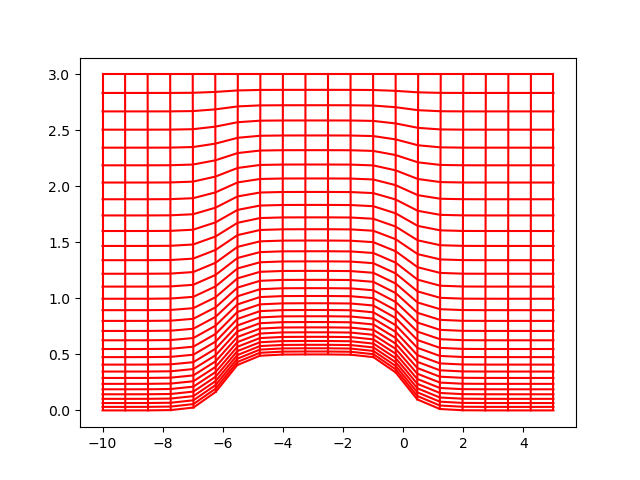
\includegraphics[width=0.8\textwidth]{lab3/Figure1.png}
    \caption{a 30x20 grid skewed by a factor $\delta=1.5$}
    \label{fig:grid}
\end{figure}

We implemented also this \texttt{Domain}-class as specified, with the grid being generated with a stretch in the y-direction. The resulting grid generated for $30\times 20$ nodes can be seen in figure \ref{fig:grid}. Generating a $1000\times 1000$ grid on a 12 core machine takes about 60 seconds, which seems like an acceptable time.


\section{Code structure}
All the code can be found at \href{https://github.com/jonasnylund/SF2565-CPP}{https://github.com/jonasnylund/SF2565-CPP} in the folder for \texttt{lab3}. The code header files are located in the \texttt{include/} folder, the source code in \texttt{src/} and \texttt{bin/} is for binary output files. Running \texttt{make} produces a output program file \texttt{main}, assuming a Linux-compatible system.

\subsection*{Curvebase.hpp}
Base class for space curves.
\lstinputlisting[language=C++]{include/Curvebase.hpp}


\subsection*{Line.hpp}
Class for a basic straight line. Extends \texttt{Curvebase} and is used for the straight sides of the domain.
\lstinputlisting[language=C++]{include/Line.hpp}


\subsection*{ExpBulge.hpp}
Class for representing the non-straight lower boundary of the domain. Also inherits from \texttt{Curvebase}
\lstinputlisting[language=C++]{include/ExpBulge.hpp}

\subsection*{Domain.hpp}
Class for representing the domain. The grid is generated by calling \texttt{generate\_grid(int, int, double)}, where the first two arguments are the grid size in y and x-directions respectively, and the last argument is the stretching of the grid i y. The file is written to disk by the \texttt{toFile(string)} method.
\lstinputlisting[language=C++]{include/Domain.hpp}

\subsection*{Main.cpp}
The grid is generated by the main program. Compile the code using \texttt{make} (Makefile included in the github repository). The first two arguments to the program are the grid size, the second is the stretching parameter $\delta$ and the last is the output filename for the generated grid to save to. 

\lstinputlisting[language=C++]{src/main.cpp}

\subsection*{Plotting the results}
To plot the produces file, run \texttt{python3 plot.py filename}, where \texttt{filename} is the name of the binary outputfile of the \texttt{main} program.
The source code is available on GitHub.

\end{document}
